\subsection{WiFi Scanning (Wardriving)}

Auch hier fand ich keine iOS Apps, die in Frage kommen (zumindest keine kostenlosen). Das in der Angabe vermerkte Programm "Wlandscape" wurde 2007 zum letzten Mal aktualisiert und war nicht ohne Exceptions verwendbar. \enquote{Inssider} ist nur für Windows verfügbar und kam daher auch nicht in Frage.

Also führte ich auch hier die Messungen mit meinem Tablet durch. Die App \enquote{Wifi Tracker} war im Play Store nicht verfügbar, eine im Internet herunterladbare Version war nicht mit meinem Tablet kompatibel. Die App \enquote{NetSpot} scheint für diese Aufgabe gut geeignet zu sein, erlaubt sie doch das Aufnehmen von Bildern als Kartengrundlage. Messungen sind damit auch Möglich, die Anzeige der APs auf der Karte ist allerdings kostenpflichtig, weshalb auch diese App nicht in Frage kam.

Ein Vergleich zwischen Scans mit Mobiltelefonen und Laptops ist demnach nicht möglich gewesen.

Die Scans wurden mit der bereits oben erwähnten App \enquote{WiGLE WiFi Wardriving} von WiGLE.net auf meinem Samsung Tab S7FE durchgeführt. Die App scannt beim Herumlaufen automatisch nach APs und zeigt diese anhand der per GPS erkannten Position auf einer Karte an.

Für diese Aufgabe hat sich die App als nur bedingt geeignet herausgestellt. Die Scans wurden im Erdgeschoss der F21 durchgeführt, wobei die angezeigte Position gelegentlich herumsprang oder auf der Karte offensichtlich nicht mit der tatsächlichen Position übereinstimmte. Zusätzlich ist durch die begrenzte Auflösung der Satellitenkarte eine genaue Bestimmung der Positionsunterschiede der APs nicht sinnvoll möglich.

Die Scans offenbarten eine Vielzahl von APS, von denen manche, aber nicht alle, auch offensichtlich im Flur montiert waren. Hier hat die Position oft grob gestimmt, wenn nicht das GPS Signal meine Position gerade offensichtlich außerhalb des Gebäudes angezeigt hat. Dies ist auf dem Screenshot \ref{screen-wardriving} gut zu sehen. Die vielen erkannten APs im Innenhof des Gebäudes sind wohl alle auf inkorrektes GPS Signal zurückzuführen, im linken Flügel des Gebäudes sind kaum APs erkannt worden, obwohl dort auch welche montiert sind. Die APs im rechten Flügel sind aber grob korrekt, insbesondere der Hervorgehobene.

\begin{figure}[h]
    \centering
    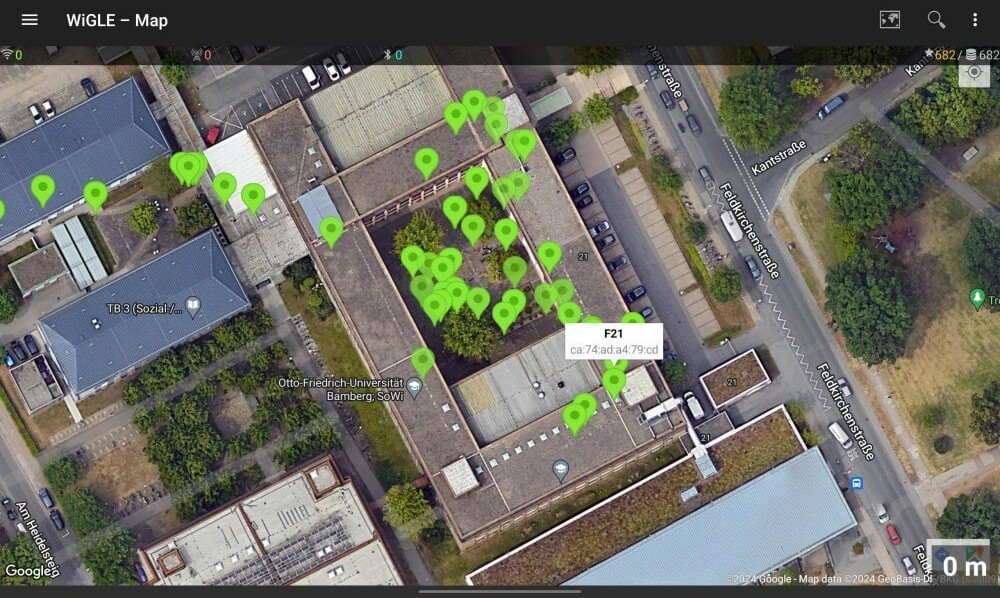
\includegraphics[width=0.9\textwidth]{figures/screen-wardriving.jpg}
    \caption{Screenshot der WiGLE WiFi Wardriving App. Die grünen Punkte sind alles erkannte APs.}
    \label{screen-wardriving}
\end{figure}

Mehrere Wiederholungen zeigten grob ähnliche Positionen, aber auch hier ist keine genauere Bestimmung durch die Ungenauigkeiten des GPS Signals und der Karte möglich.

Gut zu sehen ist auf Foto \ref{screen-wardriving-path} der gelb hinterlegte Pfad, den ich während des Scans angeblich zurückgelegt haben soll. Deutlich zu erkennen hier der um viele Meter nach oben in den Innenhof verschobene Pfad, der durch das GPS Signal verursacht wurde.

\begin{figure}[h]
    \centering
    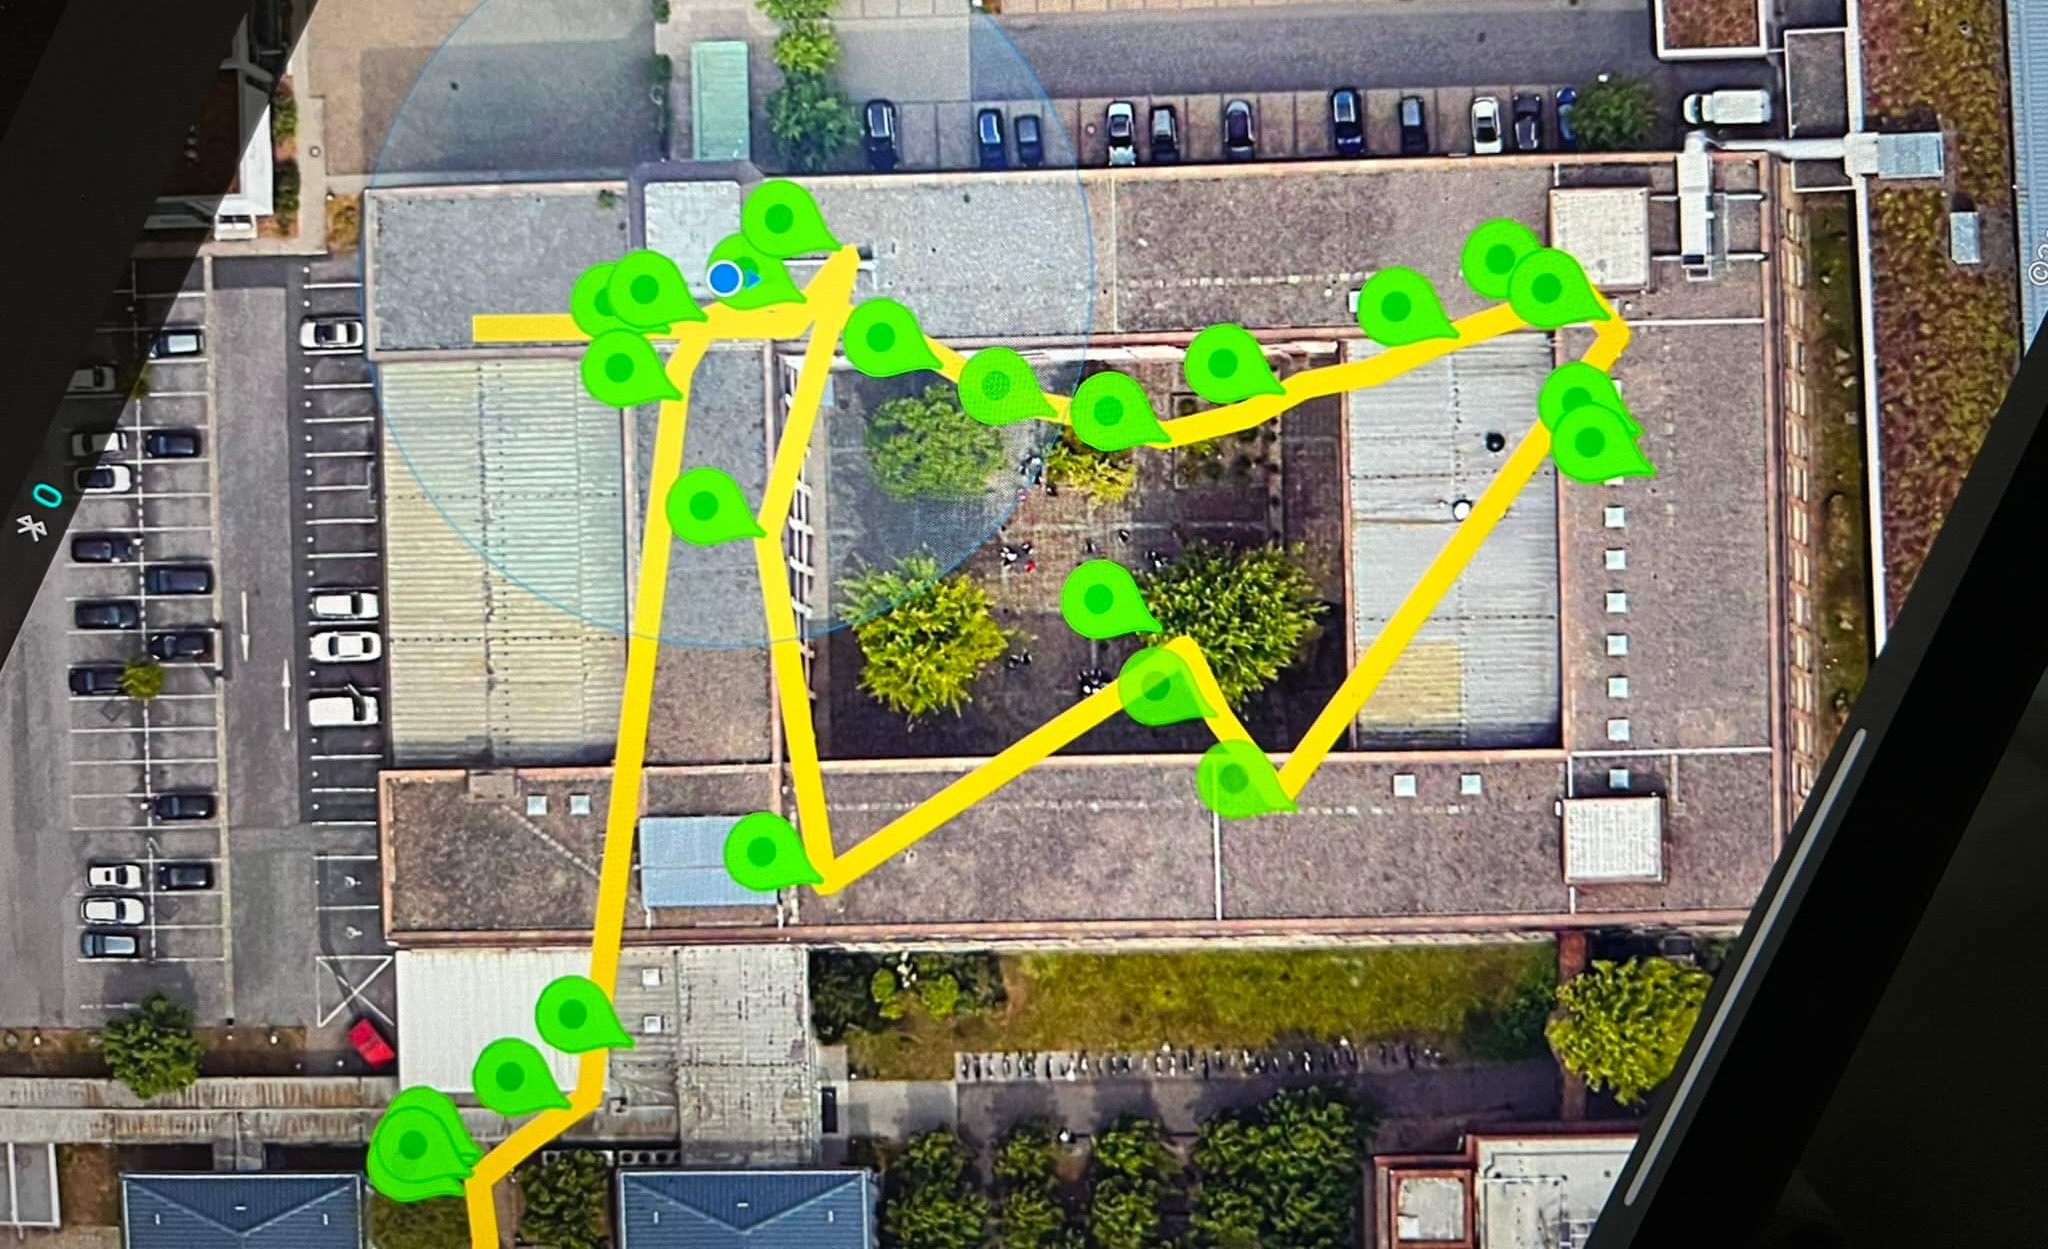
\includegraphics[width=0.8\textwidth]{figures/screen-wardriving-path.jpg}
    \caption{Foto währen des Scanprozesses. Im Vergleich zu Abbildung \ref{screen-wardriving} um etwa 45 Grad gedreht.}
    \label{screen-wardriving-path}
\end{figure}
